\documentclass[a4paper, czech]{article}

\title{
	\begin{framed}
		\setstretch{1.5}
		{\large Audio elektronika (BPC/BKC-AUD)}\\
		Laboratorní úloha č. 6 (protokol)\\
		\textbf{Digitální zpracování nízkofrekvenčního signálu}
	\end{framed}
	}
\author{Karolína A. Šebestová}
\date{24. 3. 2026, 11:00}

\usepackage[czech]{babel}
\usepackage{indentfirst}
\usepackage{graphicx}
\usepackage{float}
\usepackage[margin=1.5cm]{geometry}
\usepackage{booktabs}
\usepackage{amsmath}
\usepackage{multirow}
\usepackage{colortbl}
\usepackage{framed} % \begin{framed}
\usepackage{setspace} % \setstretch{}
\usepackage{siunitx}
\usepackage{xcolor}
\usepackage{subcaption}
%\usepackage{caption}

\sisetup{locale = DE}


\begin{document}

\maketitle

\section{Výsledky měření}

\subsection{Vliv stupně konverze (délky slova)}

\begin{figure}[H]
	\centering
	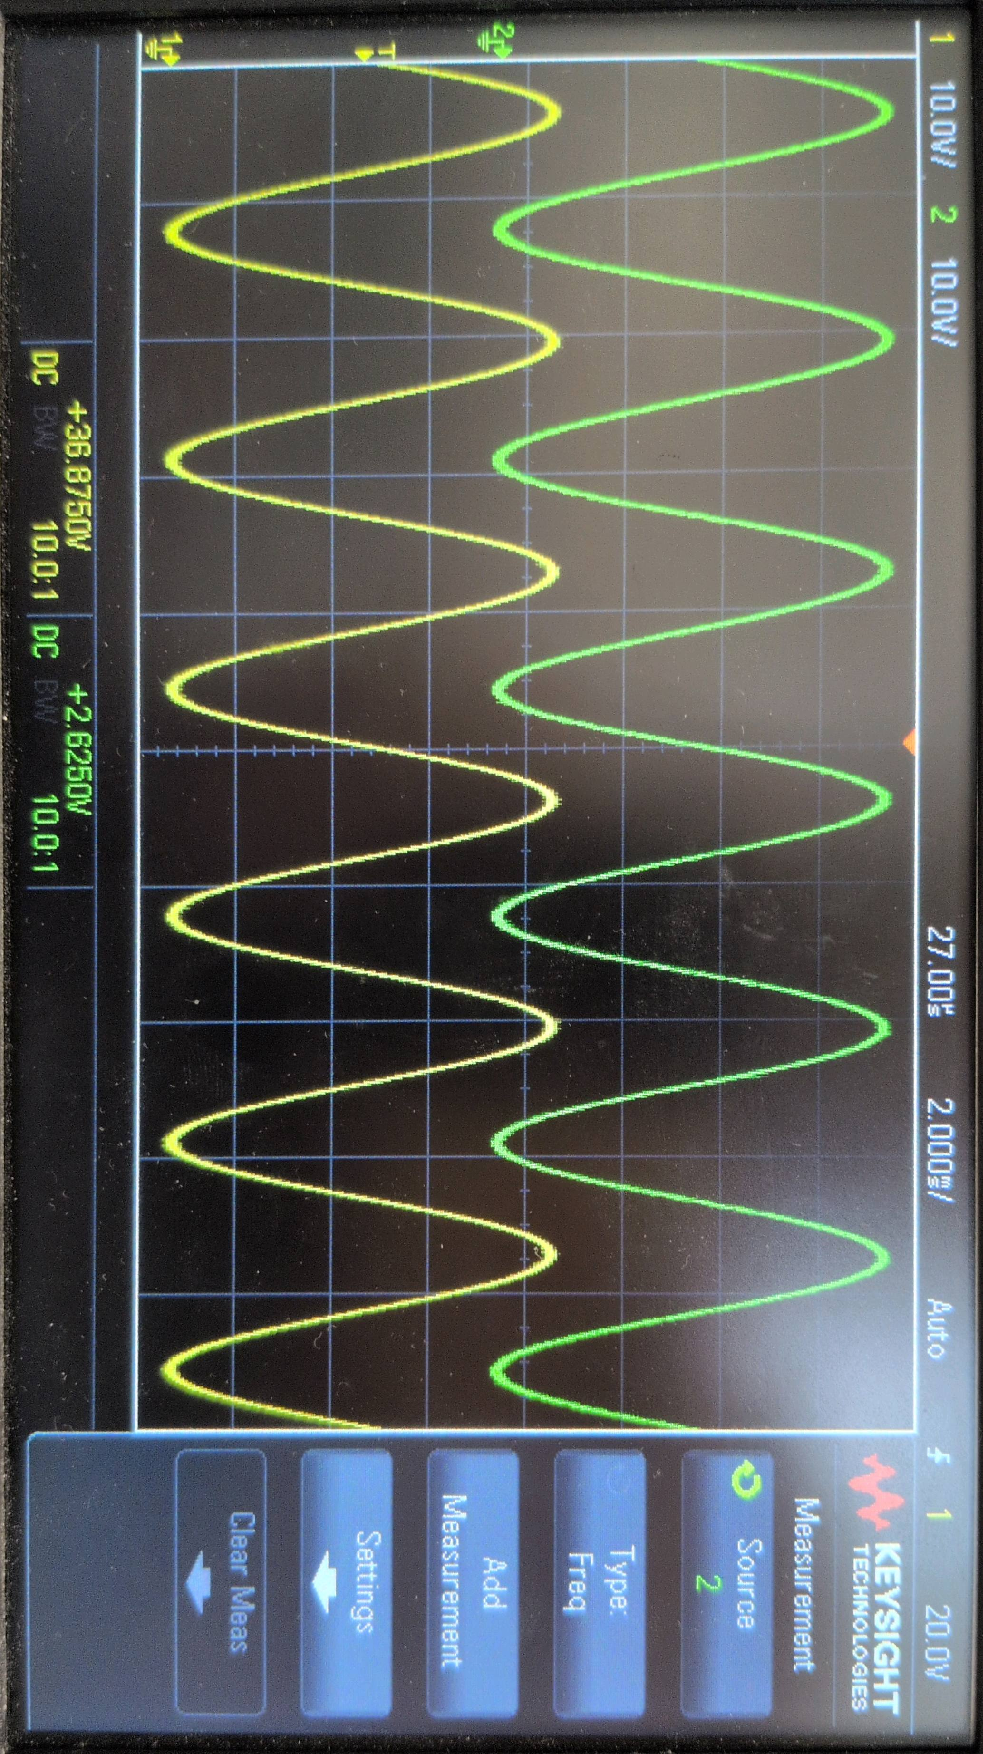
\includegraphics[height=0.7\textwidth, angle=90, page=1]{osciloskop/1_vliv_stupne_konverze.pdf}
	\caption{Vliv stupně konverze na přesnos signálu: \textbf{8 bitů}.}
\end{figure}

\begin{figure}[H]
	\centering
	\includegraphics[height=0.7\textwidth, angle=90, page=2]{osciloskop/1_vliv_stupne_konverze.pdf}
	\caption{Vliv stupně konverze na přesnos signálu: \textbf{6 bitů}.}
\end{figure}

\begin{figure}[H]
	\centering
	\includegraphics[height=0.7\textwidth, angle=90, page=3]{osciloskop/1_vliv_stupne_konverze.pdf}
	\caption{Vliv stupně konverze na přesnos signálu: \textbf{4 bity}.}
\end{figure}

\begin{figure}[H]
	\centering
	\includegraphics[height=0.7\textwidth, angle=90, page=4]{osciloskop/1_vliv_stupne_konverze.pdf}
	\caption{Vliv stupně konverze na přesnos signálu: \textbf{3 bity}.}
\end{figure}

\subsection{Vliv změny vzorkovacího kmitočtu}

\begin{figure}[H]
	\centering
	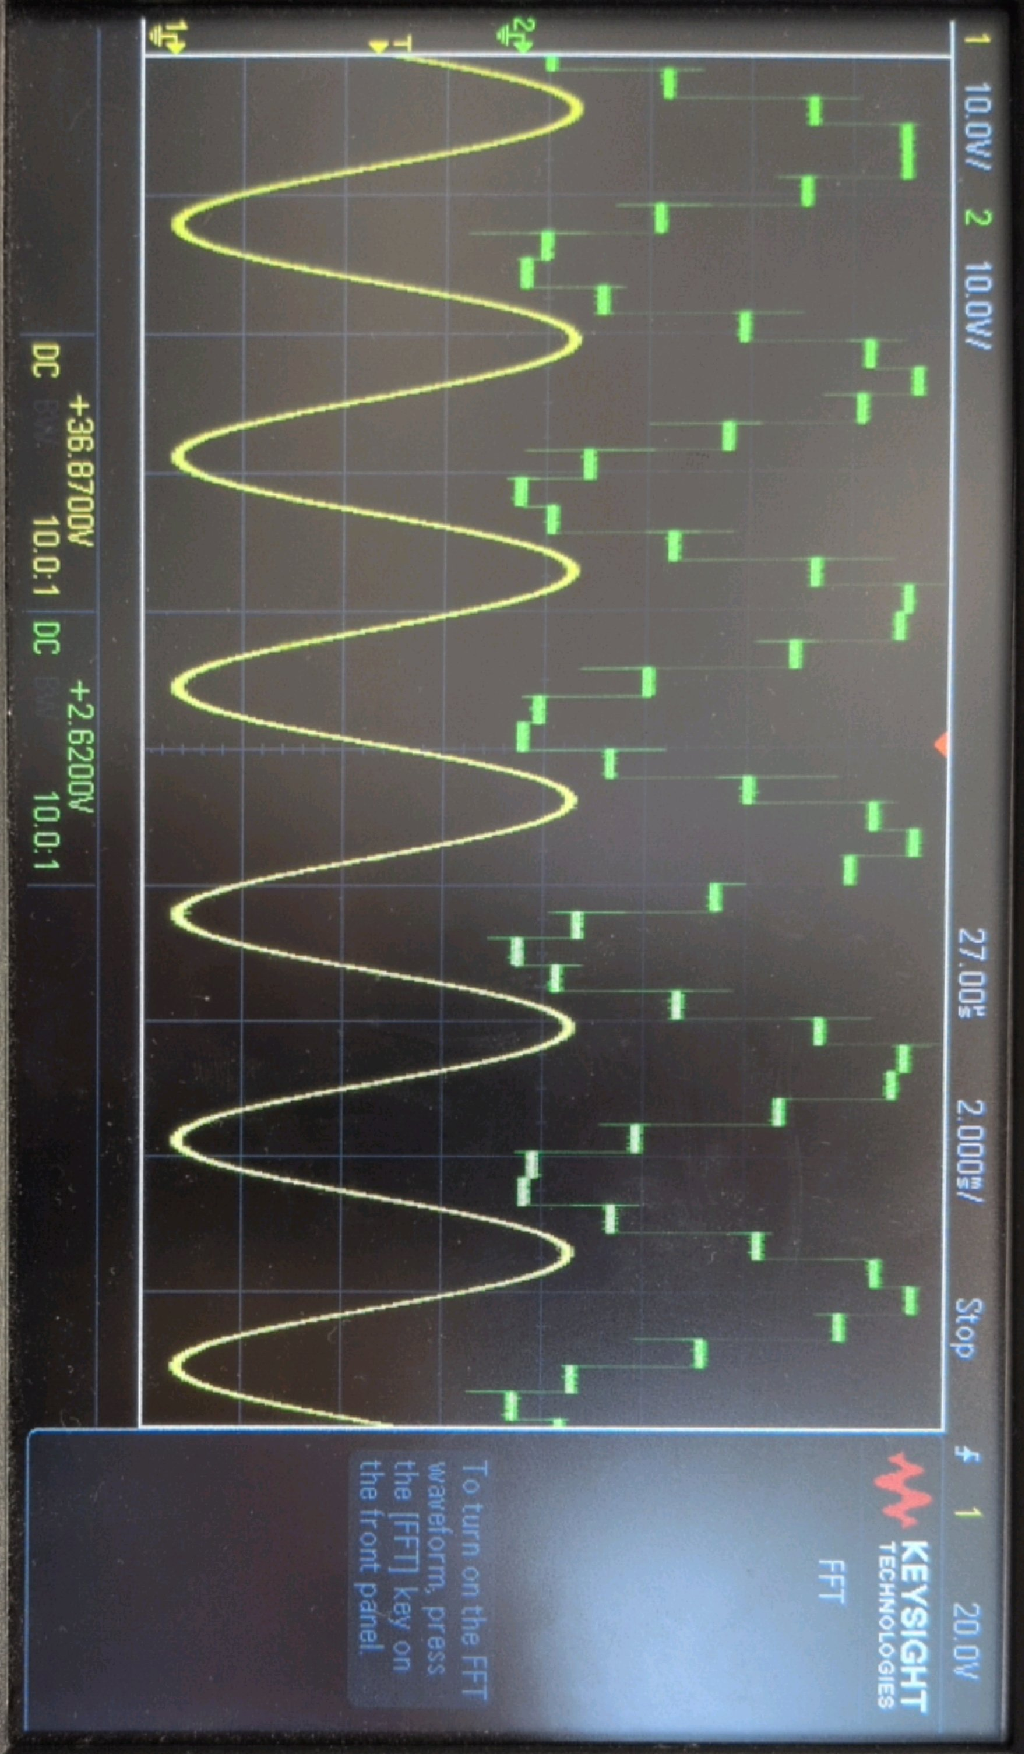
\includegraphics[height=0.7\textwidth, angle=90, page=1]{osciloskop/2_vliv_zmeny_vzorkovaciho_kmitoctu.pdf}
	\caption{Přenos harmonického signálu při vzorkovacím kmitočtu $\sim 5$\,kHz s 8-bitovým rozlišením.}
\end{figure}

\subsection{Vliv výstupního filtru}

\begin{figure}[H]
	\centering
	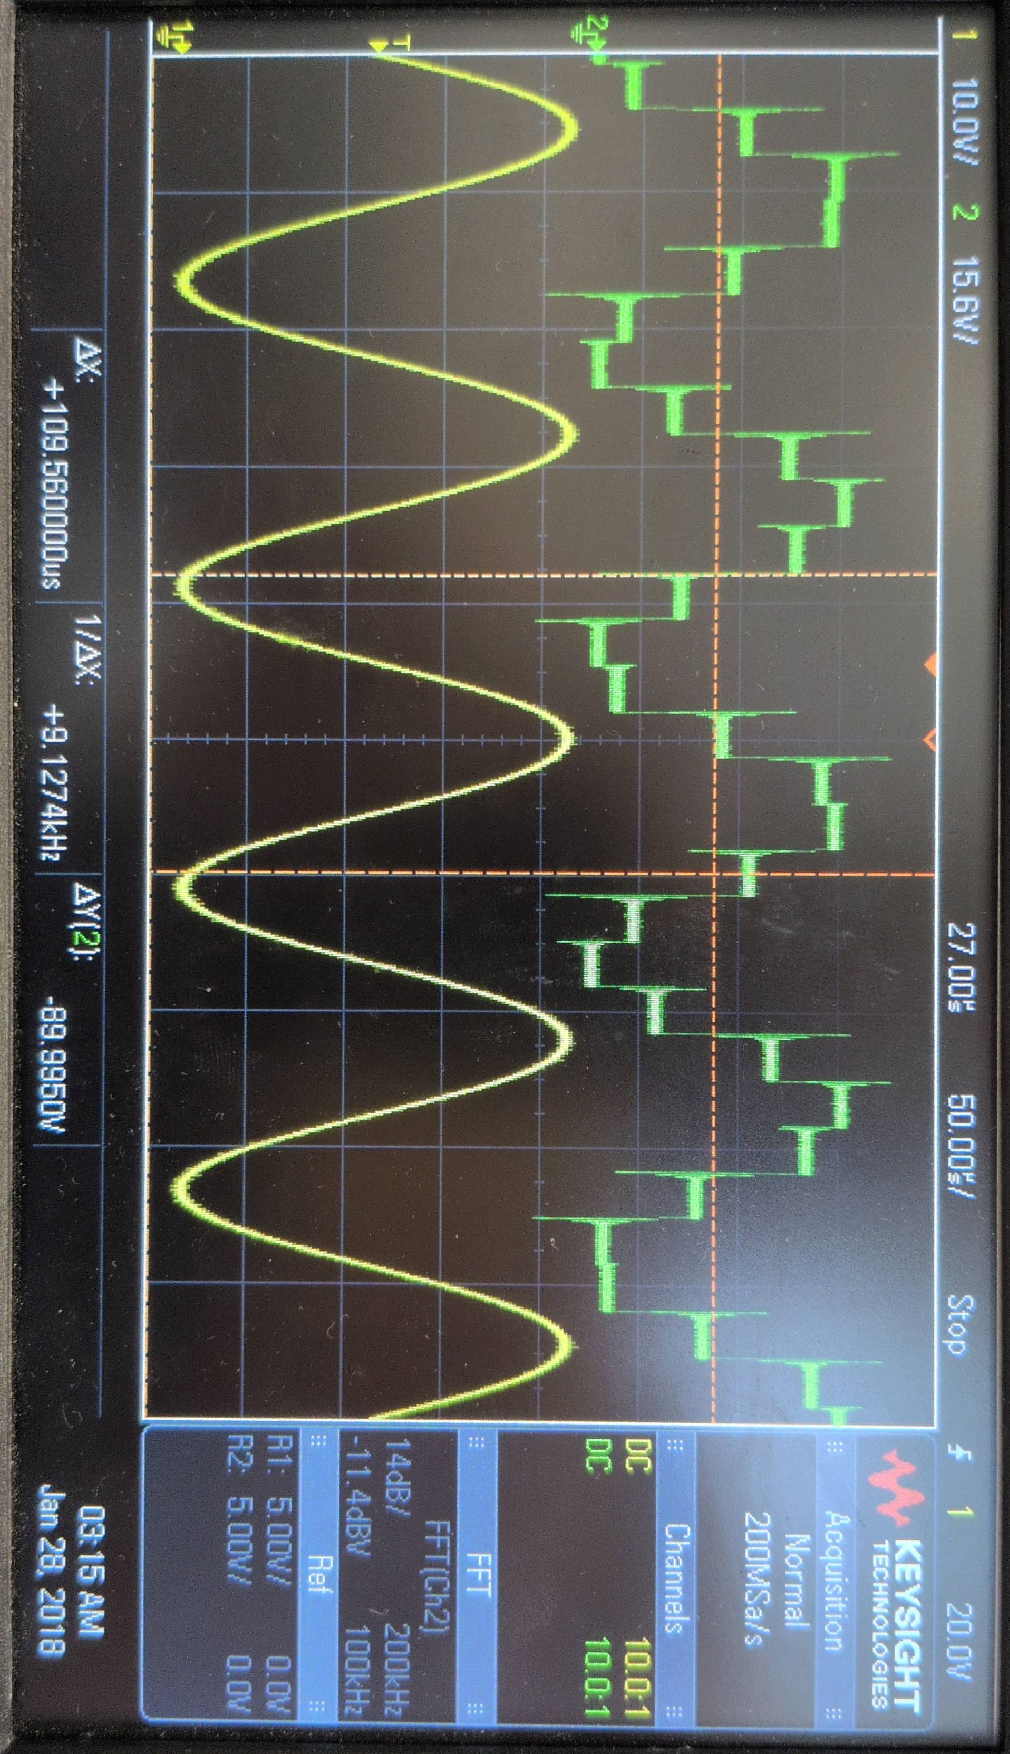
\includegraphics[height=0.7\textwidth, angle=90, page=1]{osciloskop/3_vystupni_filtr_2.pdf}
	\caption{Vliv výstupního filtru na přenos harmonického signálu o frekvenci blízké $fvz/2$ - \textbf{filtr vypnut}.}
\end{figure}

\begin{figure}[H]
	\centering
	\includegraphics[height=0.7\textwidth, angle=90, page=2]{osciloskop/3_vystupni_filtr_2.pdf}
	\caption{Vliv výstupního filtru na přenos harmonického signálu o frekvenci blízké $fvz/2$ - \textbf{filtr zapnut}.}
\end{figure}

\subsection{Vznik degradace harmonického signálu}

\begin{figure}[H]
	\centering
	\includegraphics[height=0.7\textwidth, angle=90, page=2]{osciloskop/4_degradace .pdf}
	\caption{Degradace vstupního harmonického signálu na signál obdélníkový.}
\end{figure}

\subsection{Vznik a velikost kvantizačního zkreslení}

\begin{figure}[H]
	\centering
	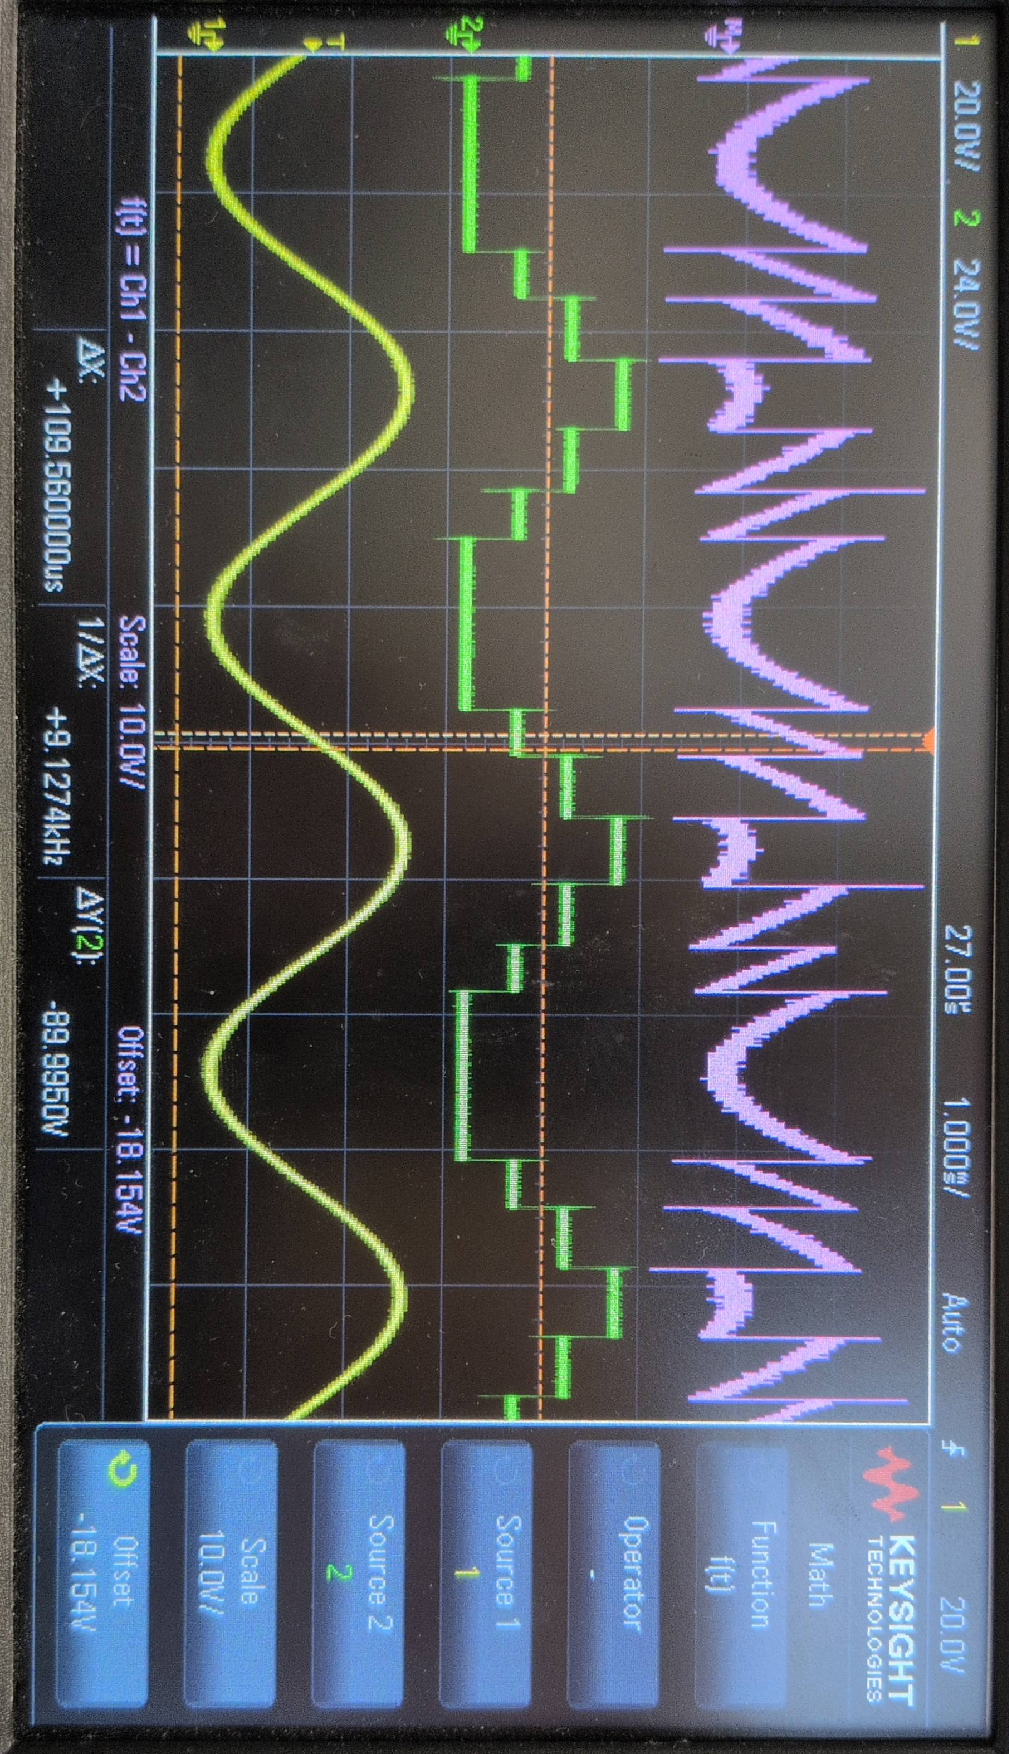
\includegraphics[height=0.7\textwidth, angle=90, page=1]{osciloskop/5_kvantizacni_zkresleni.pdf}
	\caption{Kvantizační zkreslení - rozlišení \textbf{3 bity}.}
\end{figure}

\begin{figure}[H]
	\centering
	\includegraphics[height=0.7\textwidth, angle=90, page=2]{osciloskop/5_kvantizacni_zkresleni.pdf}
	\caption{Kvantizační zkreslení - rozlišení \textbf{4 bity}.}
\end{figure}

\begin{figure}[H]
	\centering
	\includegraphics[height=0.7\textwidth, angle=90, page=3]{osciloskop/5_kvantizacni_zkresleni.pdf}
	\caption{Kvantizační zkreslení - rozlišení \textbf{6 bitů}.}
\end{figure}

\begin{figure}[H]
	\centering
	\includegraphics[height=0.7\textwidth, angle=90, page=4]{osciloskop/5_kvantizacni_zkresleni.pdf}
	\caption{Kvantizační zkreslení - rozlišení \textbf{8 bitů}.}
\end{figure}

\subsection{Vznik granulačního zkreslení}

\begin{figure}[H]
	\centering
	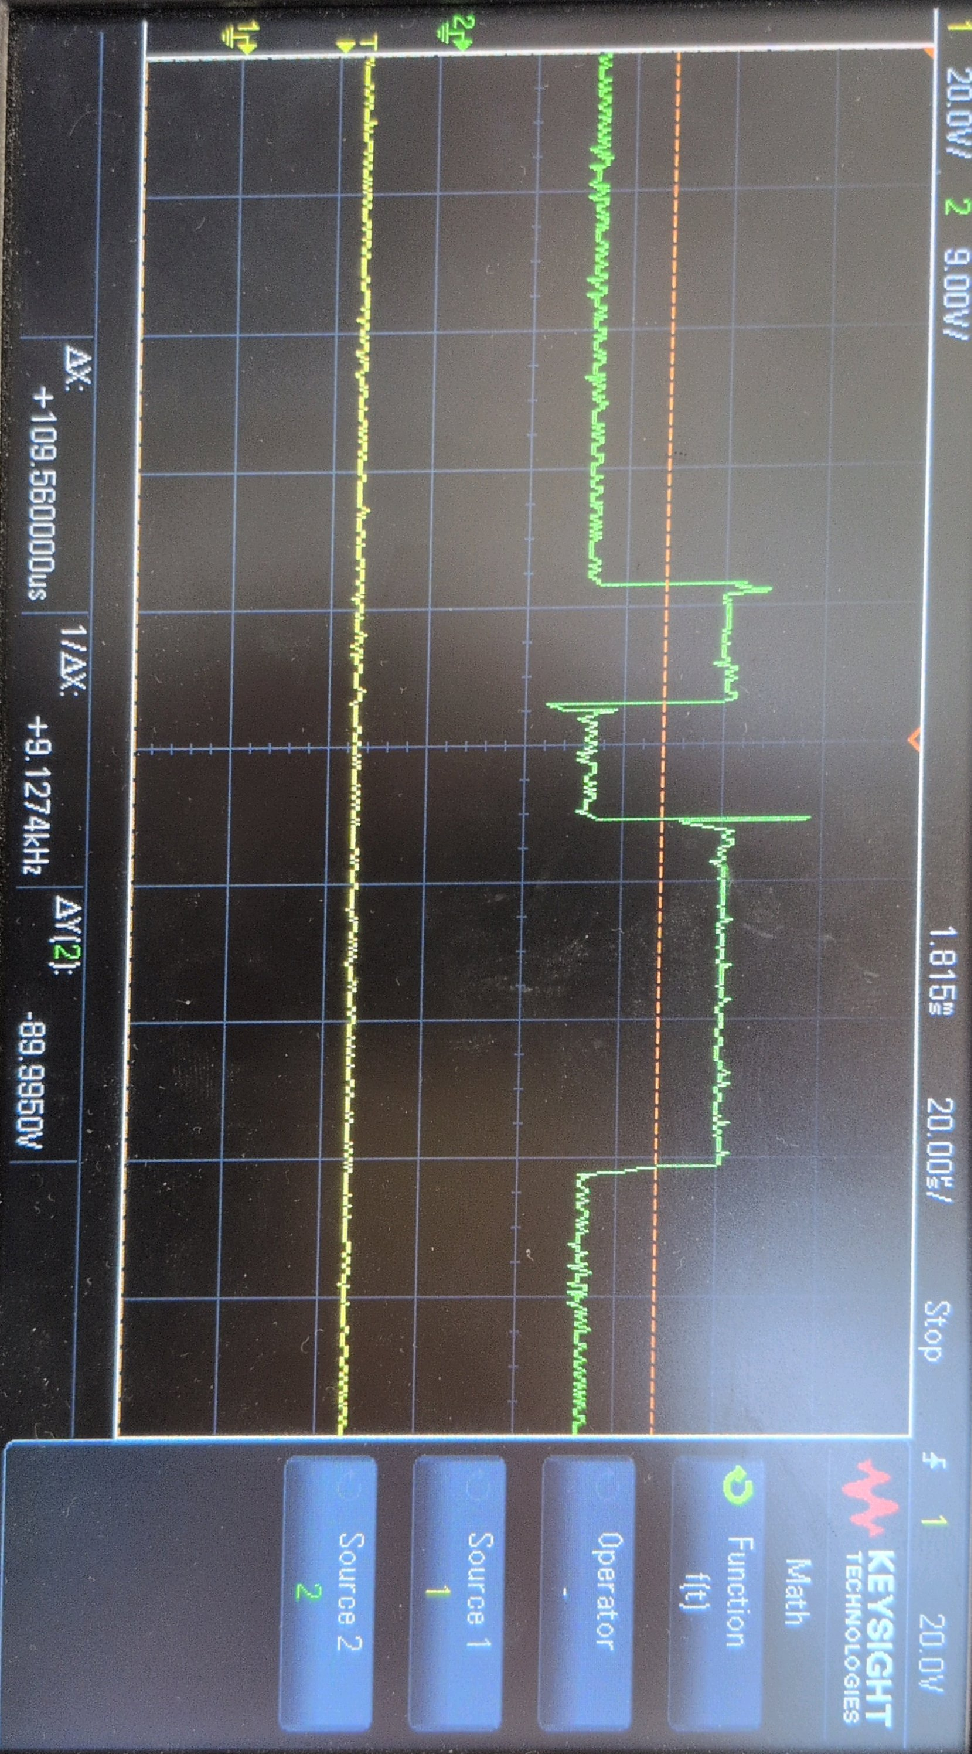
\includegraphics[height=0.7\textwidth, angle=90, page=1]{osciloskop/6_granulacni_zkresleni.pdf}
	\caption{Přiblížení granulačního zkreslení.}
\end{figure}

\subsection{Zákmity na hranách výstupního signálu}

\begin{figure}[H]
	\centering
	\includegraphics[height=0.7\textwidth, angle=90, page=2]{osciloskop/7_zákmity.pdf}
	\caption{Přiblížení zákmitů na hranách výstupního signálu}
\end{figure}

\subsection{Rozšíření kmitočtového spektra}

\begin{figure}[H]
	\centering
	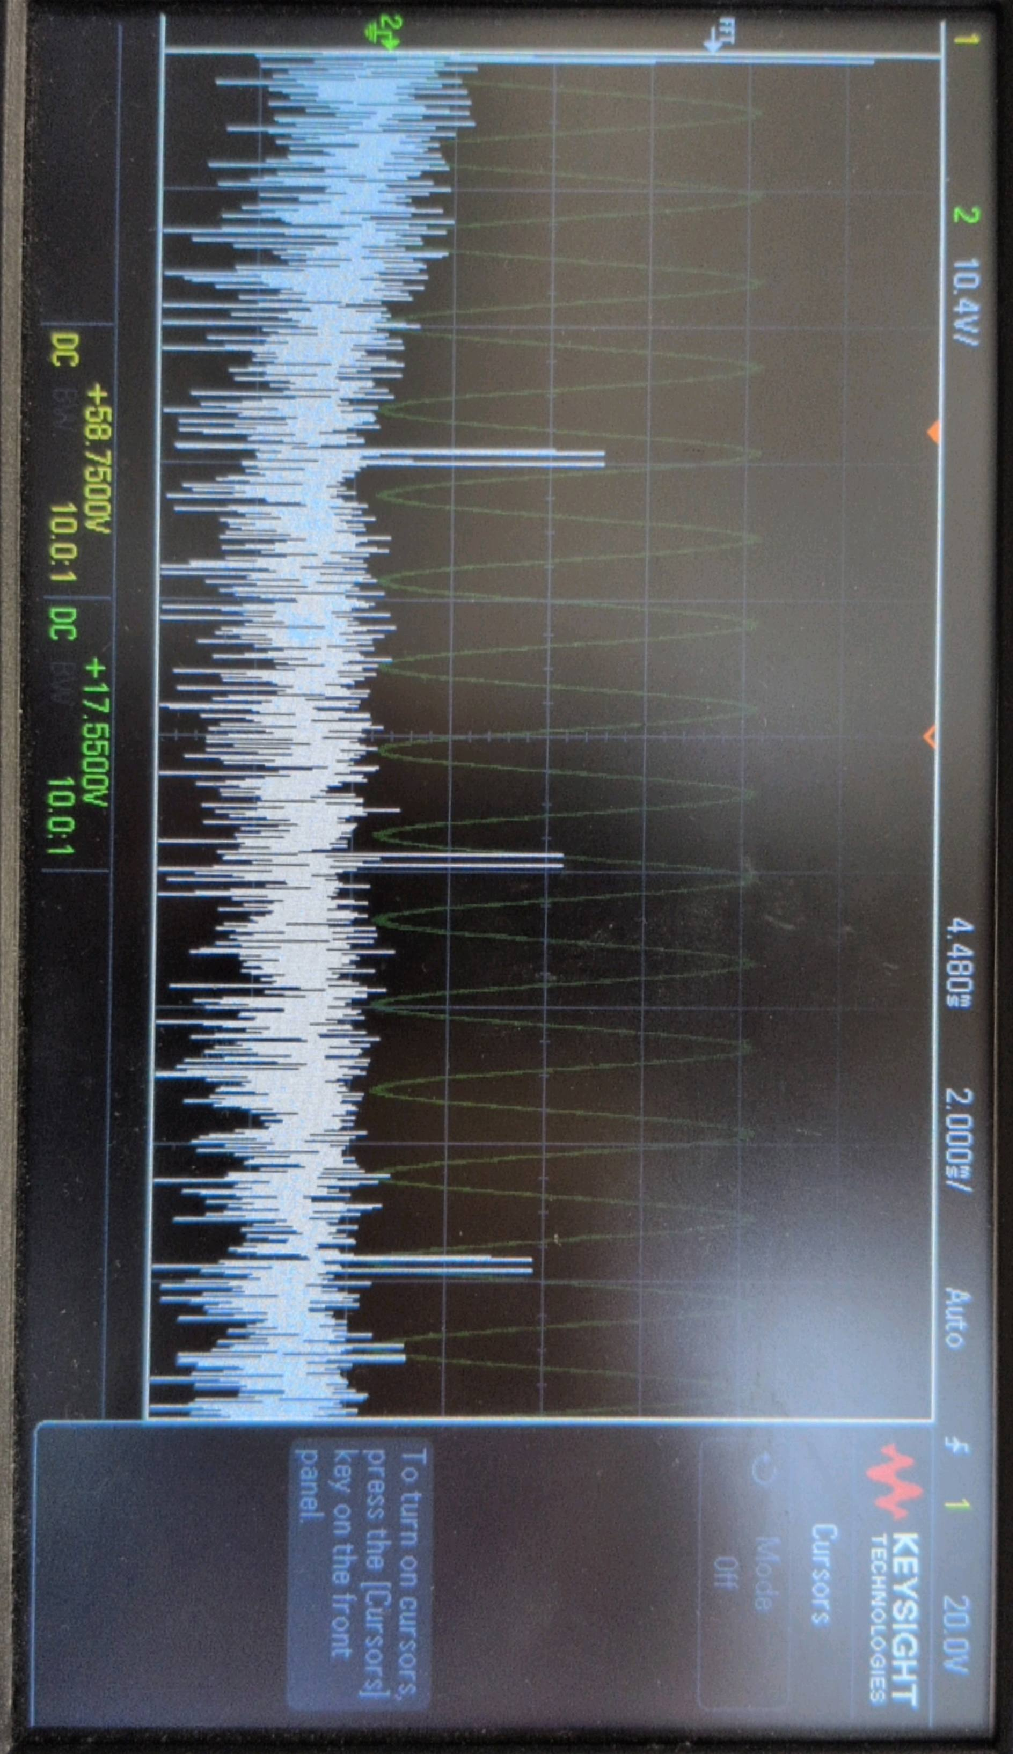
\includegraphics[height=0.7\textwidth, angle=90, page=1]{osciloskop/8_rozsireni_spektra_2.pdf}
	\caption{Kmitočtové spektrum při dodržení Shannon-Kotělnikova teorému.}
\end{figure}

\begin{figure}[H]
	\centering
	\includegraphics[height=0.7\textwidth, angle=90, page=2]{osciloskop/8_rozsireni_spektra_2.pdf}
	\caption{Rozšíření kmitočtového spektra při nedodržení Shannon-Kotělnikova teorému.}
\end{figure}

\subsection{Vznik aliasingu}

\begin{figure}[H]
	\centering
	\includegraphics[height=0.7\textwidth, angle=90, page=2]{osciloskop/9_aliasing.pdf}
	\caption{Vznik aliasingu při kmitočtu vyšším než $f_vz$.}
\end{figure}

\section{Použité měřící přístroje}

\begin{itemize}
    \item \textbf{GEN} nízkofrekvenční funkční generátor Digimess FG100
    \item \textbf{OSC} paměťový osciloskop HP 54603A 60 MHz
    \item \textbf{NZ} napájecí zdroj Diametral (napájení $\pm$ 15V, +5V)
    \item \textbf{LPT} tiskárna HP 5L připojená k osciloskopu
    \item měřený přípravek „Digitální zpracování nízkofrekvenčních signálů“
    \item propojovací vodiče 3 x BNC – BNC, 1 x rozbočovací „T člen“
\end{itemize}

\section{Závěr}

\end{document}